\section{Correlation Regime Changes}
Rolling 60-day correlations show clear regime changes:
\begin{itemize}
  \item S\&P vs UST10 ranges from \(-0.48\) to \(+0.79\), indicating sign flips.
  \item CDX IG vs UST10 ranges from \(-0.82\) to \(+0.48\), another clear breakdown from stable one-sign relationships.
  \item CDX IG vs S\&P remains negative throughout but weakens materially in some windows (from about \(-0.92\) to \(-0.27\)).
\end{itemize}

Economic interpretation:
\begin{itemize}
  \item During acute stress windows, rates and credit can move together as policy expectations and growth fears dominate simultaneously.
  \item In inflation-driven tightening regimes, rates can rise while growth-sensitive assets struggle, changing conventional sign patterns.
  \item Liquidity and technical flows can temporarily dominate macro betas, especially around major event windows.
\end{itemize}

\begin{figure}[H]
  \centering
  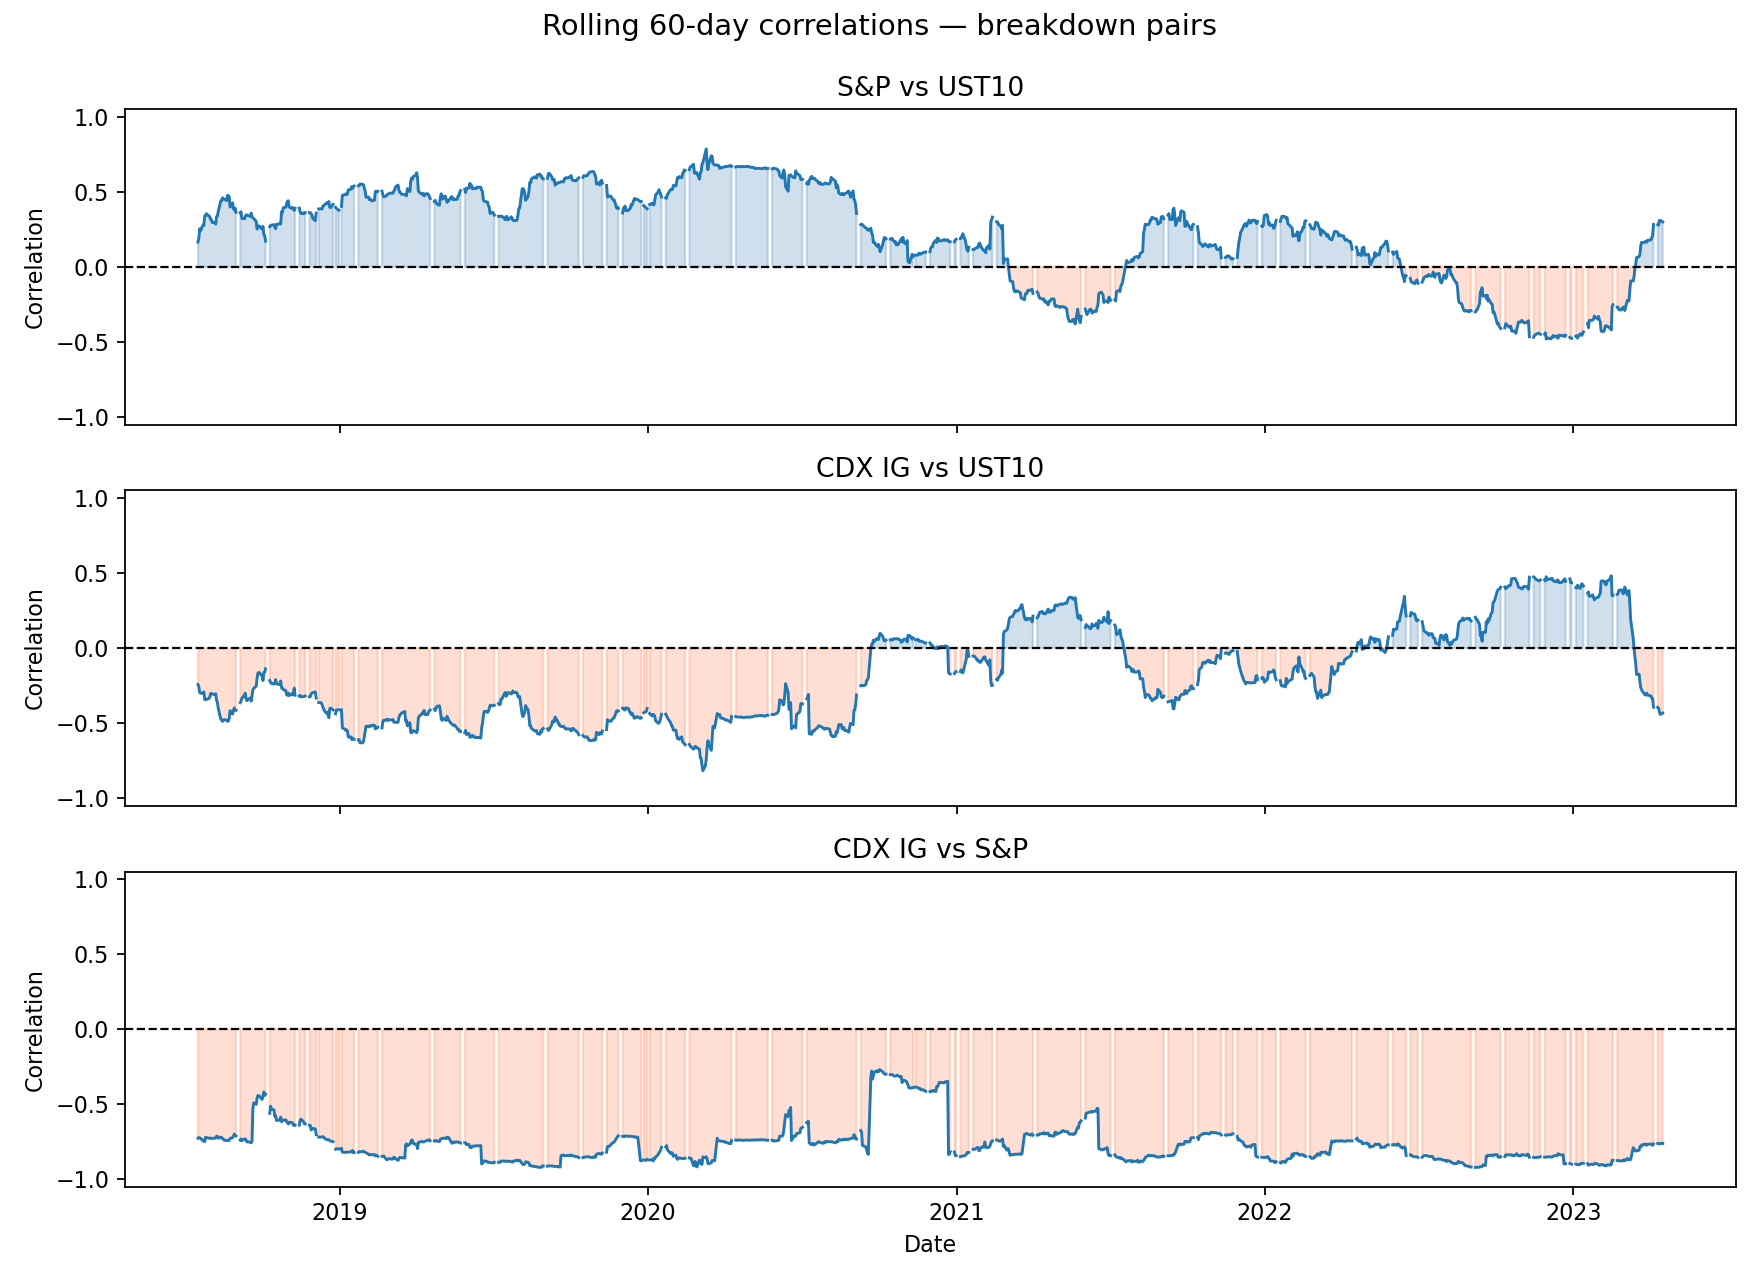
\includegraphics[width=\textwidth]{../../../output/figures/rolling_correlations.png}
  \caption{Rolling 60-day correlations for the three pairs exhibiting sign flips or material breakdowns. Positive regions shaded in blue, negative in red.}
\end{figure}
